\documentclass{article}

\usepackage{arxiv/arxiv}

\usepackage[utf8]{inputenc} % allow utf-8 input
\usepackage[T1]{fontenc}    % use 8-bit T1 fonts
\usepackage{hyperref}       % hyperlinks
\usepackage{url}            % simple URL typesetting
\usepackage{booktabs}       % professional-quality tables
\usepackage{amsfonts}       % blackboard math symbols
\usepackage{nicefrac}       % compact symbols for 1/2, etc.
\usepackage{microtype}      % microtypography
\usepackage{cleveref}       % smart cross-referencing
\usepackage{lipsum}         % Can be removed after putting your text content
\usepackage{graphicx}
\usepackage{natbib}
\usepackage{doi}
\usepackage{makecell}

\title{High Dynamic Range Image(HDRI) Estimation Method }

\author{
    \hspace{1mm}Zihang Zhu \\
    Nanjing University
}

\hypersetup{
    pdftitle={hdri_estimation_method},
    pdfsubject={q-bio.NC, q-bio.QM},
    pdfauthor={Zihang Zhu},
    pdfkeywords={HDRI, Inverse},
}

\begin{document}
\maketitle

\begin{abstract}
    High Dynamic Range (HDR) image is vastly used for environment lighting in renderers and game engines. \\
    However, estimating HDR image from synthetic low dynamic range (LDR) and limited field of view (LFOV) image(s) is a still a challenging problem.
\end{abstract}

% keywords can be removed
\keywords{HDRI \and Lighting estimation}

\section{Introduction}

\subsection{High Dynamic Range Image as Environment Lighting}

\paragraph{high dynamic range} (HDR) is a series of image format that can express
more real-world illumination information rather than low dynamic range (LDR) images like RGB.

A natural light source like the sun is actually a specturm of light [Figure \ref{fig:spectrum-of-solar-radiation}] that can be
expressed as an infinite dimension vector space by function of wavelengths.
However, when we express it in RGB format, we have to choose three limited base spectrum,
with 256 levels of radiance with minimum and maximum value for each.

\begin{figure}
    \centering
    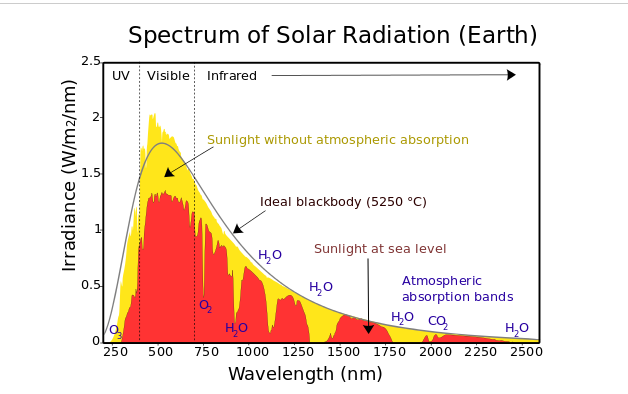
\includegraphics[width=0.8\linewidth]{spectrum-of-solar-radiation.png}
    \caption{Spectrum of Solar Radiation, from \texttt{https://www.e-education.psu.edu/meteo300/node/683}}
    \label{fig:spectrum-of-solar-radiation}
\end{figure}

Display devices for digital images, such as computer monitors and video projectors,
usually have a dynamic range of about 500 to 1, which means the brightest pixel in an image is never more than
500 time brighter than the darkest pixel.
Thus, the normal RGB formats, which are often designed for those devicees,
are not suitable for expressing the real-world illumination information,
as shown in [Figure \ref{fig:dynamic-range}],
which is the reason why HDR image format is invented.

\begin{figure}
    \centering
    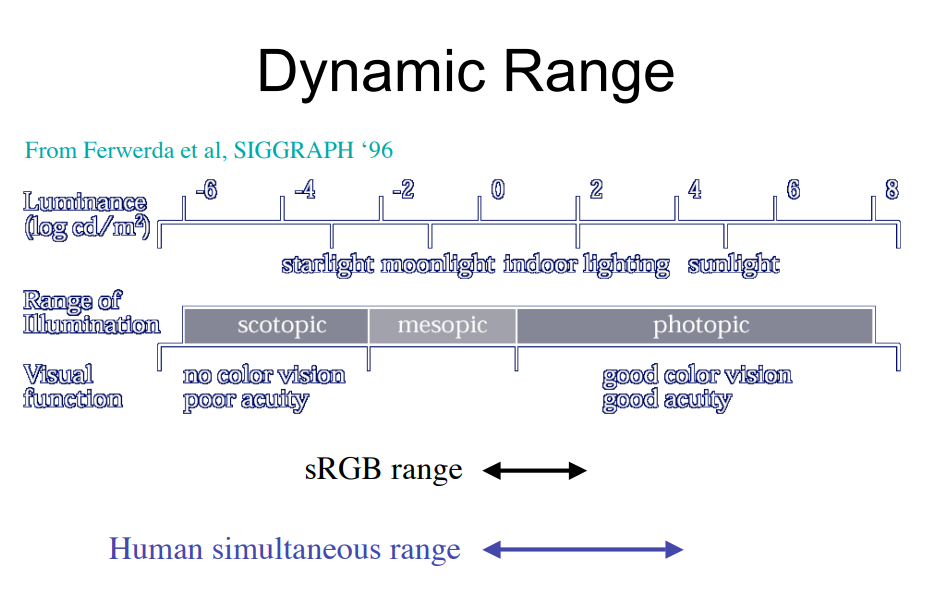
\includegraphics[width=0.8\linewidth]{dynamic_range.png}
    \caption{Dynamic Range for Colors}
    \label{fig:dynamic-range}
\end{figure}


A typical HDR file format, .exr, as an example, will store each RGBA pixels into 16 or 32 bit floating piont numbers.
Even with 16-bit floating-point numbers,
color resolution is 1024 steps per f-stop,
as opposed to somewhere around 20 to 70 steps per
f-stop for most 8-bit file format (.png, .jpg, etc.). see \texttt{https://openexr.com/en/latest/TechnicalIntroduction.html} for more information.



\paragraph{image-based lighting} (IBL) [\cite{wardHighDynamicRange2008}]
is the process of illuminating scenes and objects (real or synthetic)
with images of light from real world.

It envolved from the reflection-mapping technique[
        \cite{millerIlluminationReflectionMaps1984}
        \cite{blinnTextureReflectionComputer1976}]
, where the graphics scientists use a panorama image as a texture to simulate the reflected light information
on the surface of the object.

in 2002, scientists found that the high-dynamic-range images are very suitable
for IBL[\cite{debevecRenderingSyntheticObjects1998}], espetially for complex environment lighting like outdoor scenes
    [\cite{durandFastBilateralFiltering2002},
        \cite{fattalGradientDomainHigh2002},
        \cite{reinhardPhotographicToneReproduction2002}].

Till now, using HDRI as environment lighting is a common feature for most popular
renderers and game engines, such as
Blender \footnote{\texttt{https://docs.blender.org/manual/zh-hans/latest/render/lights/world.html}},
Unity \footnote{\texttt{https://docs.unity3d.com}},
and Unreal Engine \footnote{\texttt{https://docs.unrealengine.com/4.26/zh-CN/BuildingWorlds/LightingAndShadows/HDRIBackdrop/}}, etc.

\subsection{Light Estimation and Inverse Rendering Problem}

Based on the introdution above, we may find that HDR image is nothing but a way
of expressing environment lighting. HDR images play as role of environment lighting source,
as shown in [Figure \ref{fig:environment-map}]. Thus the mission of generating HDRI is equivalent to
estimate the environment lighting from the synthetic image,
which is kind of inverse procedure for common forward rendering pipeline.

\begin{figure}
    \centering
    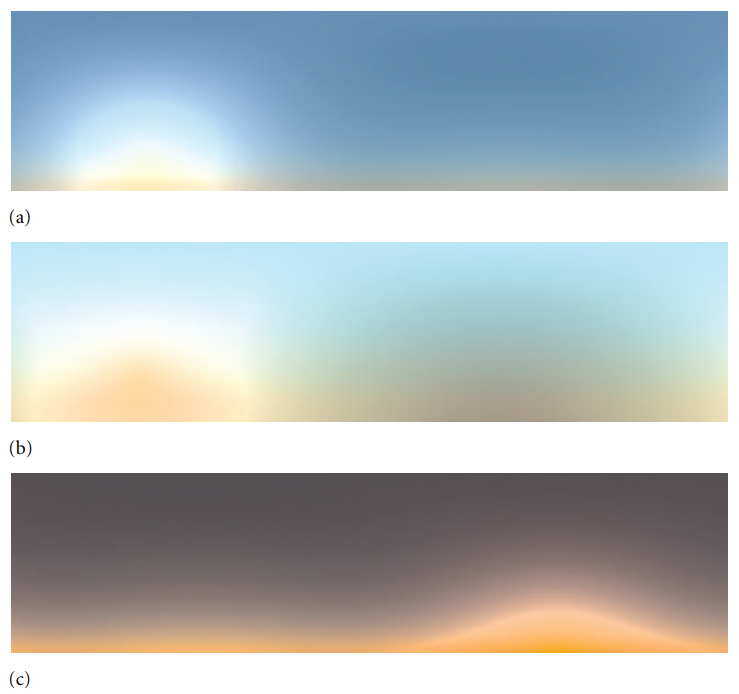
\includegraphics[width=0.6\linewidth]{environment-map.png}
    \caption{Environment Mapping for Morning, Midday and evening, from pbrt book}
    \label{fig:environment-map}
\end{figure}

It is complex to render an image from various kinds of resources, we have to define different light sources,
objects' geometry, materials and camera parameters, and implement rasterization or ray-tracing algorithns upon them.
Fortunately, the forward-porcess is determinant, different input will generate its unique output.
However, the inverse problem is not the case, for example, different geometries may result in same
synthetic images (for some may be occluded by others),
which makes it hard or even impossible to recover the raw data from the synthetic image.



Obviously, the light estimation problem can be treated as part of inverse rendering framework,
along with other problems like material estimation, geometry estimation, etc.

\subsection{The Main Challenge of HDRI Estimation}

The main challenges of light estimation problem can be listed as follows:
\begin{itemize}
    \item limited field of view (LFOV) of the synthetic image(s) is not enough for estimating panorama image
    \item object geometry, materials and light condition are highly combined and it is hard to estimate single of them without others
    \item classic rendering procedure is not differentiable, which makes it hard to train a neural network
    \item for an unlimited image input, it is hard to determine whether it is a normal "scene" or not, where the solution could not exist
\end{itemize}

In order to overcome the difficulties above, researchers have proposed various methods.
Some would like to treat the solution as an end-to-end generative model using GAN, others
may rely on depth and light model priors to esitmate it in a inverse rendering framework.
We will discuss them in detail in the following section \ref{sec:related-work}.

\subsection{Datasets and benchmarks}

The only and most complete dataset in this field I found is the
LAVAL hdr database \footnote{\texttt{http://outdoor.hdrdb.com/}}, as shown in [Figure \ref{fig:laval_hdr_databaseq}].
This dataset contains five different senario of hdr images including
\begin{itemize}
    \item indoor: with 2100+ high resolution indoor panoramas captured using a Canon 5D mark III and a robotic panoramic tripod head.
    \item outdoor: with 205 high resolution outdoor panoramas, captured using Canon 5D mark III and a robotic panoramic tripod head.
    \item sky: from [\cite{hold-geoffroyDeepSkyModeling2019}] with 7000 panoramas from SUN360-HDR
    \item indoor-spatially-varying:
    \item face \& lighting
\end{itemize}

\begin{figure}
    \centering
    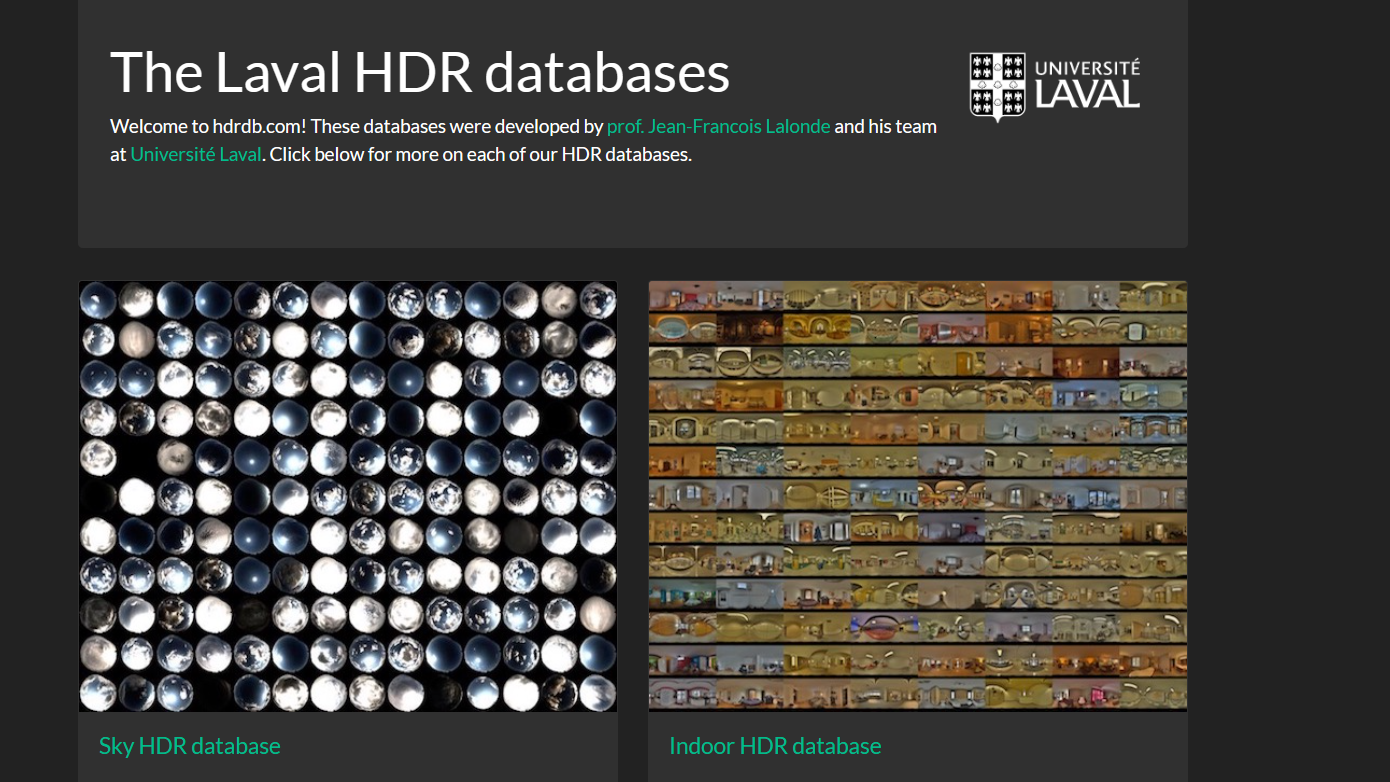
\includegraphics[width=0.8\linewidth]{laval_hdr_database.png}
    \caption{Laval HDR database, screenshot for \texttt{http://outdoor.hdrdb.com/}}
    \label{fig:laval_hdr_database}
\end{figure}

However, this dataset is restricted for acadamic use only. You have to send an email to
Prof. Jean-Francois Lalonde to sign some agreements to apply for the data.

Also, we can use some synthetic datasets or multi-view datasets as alternative.

\section{Related Work}
\label{sec:related-work}

There are mainly two kinds of approaches for light-estimation,
one is generative models like GAN, the other is a part of inverse rendering pipeline with
object geometry and material priors.

\subsection{Generate HDRI without modeling the environement}

Direct estimation often requires strong priors with constricted condition. So in the literature,
scenes like indoor, outdoor and sky are often treated individually.


\begin{table}
    \caption{Sample table title}
    \centering
    \begin{tabular}{lll}
        \toprule
        \multicolumn{2}{c}{Part}                                                                                  \\
        \cmidrule(r){1-2}
        Year\& Conference  & Type    & Brief                                                                      \\
        \midrule
        SIGGRAPH Asia 2017 & Indoor  &
        \makecell{[\cite{gardnerLearningPredictIndoor2017}]
        with lighting classifier to annotate the location, a predictor for light source and                       \\ a DNN to predict the light position, then fine-tune to HDR dataset} \\
        ECCV 2022          & Indoor  &
        \makecell{[\cite{wangStyleLightHDRPanorama2022}]
        generate HDR using double StyleGAN2}                                                                      \\
        CVPR 2019          & Outdoor &
        \makecell{[\cite{zhangAllWeatherDeepOutdoor2019}]
        use CNN to predict HDR                                                                                    \\ outdoor illumination from single LDR image. }                                                                                    \\

        3DV 2022           & Outdoor & \makecell{[\cite{dastjerdiGuidedCoModulatedGAN2022}] a 360deg FOV GAN}     \\

        CVPR 2019          & Sky     & \makecell{[\cite{hold-geoffroyDeepSkyModeling2019}] predict sky using CNN} \\

        \bottomrule
    \end{tabular}
    \label{tab:table}
\end{table}


Other methods may add some priors on the light distribution, [\cite{zhanGMLightLightingEstimation2022}] suppose the light has a spherical distribution
with Earth Mover's Loss, and its follower [\cite{zhanGMLightLightingEstimation2022}] optimize the loss.

Most recently, an arxiv [\cite{dastjerdiEverLightIndoorOutdoorEditable2023}] start to combine indoor and outdoor scene together.

Also, generating high resolution panorama image is a relevant field [\cite{yanHORIZONHighResolutionPanorama2022}]


\subsection{Light Estimation as part of Inverse Rendering}

Inverse Rendering means deducing the camera primitive, mesh, light and material
from the rendernig result: an image or video.
This is one of the eventual target for Computer Vision.

Here I only collect some of the inverse rendering papers but not thoroughly read them:

[
\cite{yuInverseRenderNetLearningSingle2018},
\cite{wuUnsupervisedLearningProbably2020},
\cite{wangLearningIndoorInverse2021},
\cite{yuOutdoorInverseRendering2021},
\cite{zhangPhySGInverseRendering2021},
\cite{wimbauerDerendering3DObjects2022},
\cite{zhangModelingIndirectIllumination2022},
\cite{panGAN2XNonLambertianInverse2022},
\cite{nimier-davidUnbiasedInverseVolume2022}
]


\bibliographystyle{unsrtnat}
\bibliography{inv_render}  %%% Uncomment this line and comment out the ``thebibliography'' section below to use the external .bib file (using bibtex) .

\end{document}
